\chapter{虚拟化架构}\label{ch:2-virtualization-architecture}

\section{架构总览}\label{sec:2-1}

RVM是专为资源受限的微控制器打造的虚拟机监视器，它能够将一颗微控制器分解成时空上互不影响的多颗虚拟微控制器。即便其中一颗虚拟微控制器发生了致命故障，其它虚拟微控制器仍然能保持正常运作，不会受到不利影响，从而有效阻止故障或安全漏洞在整个系统中的扩散。

与常见的KVM、Virtual
Box、VMWare等产品不同，RVM将微控制器的资源静态分配给各颗虚拟微控制器，其资源分配信息在系统编译时就能够确定。三个重要因素导致了这种设计：（1）绝大多数微控制器依赖于Flash存储器保存程序，缺乏加载动态运行时库的能力，（2）微控制器的资源非常少，需要极为高效地进行利用，因此很难承担动态数据结构带来的额外开销，以及（3）在关键系统中引入过多动态性可能导致系统行为难以预测。当然，在各个虚拟微控制器内部，还是可以使用动态内存分配、动态线程创建等功能的；即便这些动态行为导致虚拟微控制器故障，也不会引起其它虚拟微控制器的正常运作。

RVM与传统虚拟化解决方案的另一个不同在于其客户机运行实时操作系统（Real-Time
Operating
System，RTOS）。这些操作系统有两个特点：（1）它们要求系统时延是确定性的，（2）它们要求虚拟化的开销要非常低。常规的虚拟化解决方案往往是基于操作\footnote{或二进制}翻译的，其底层原语往往离客户机操作系统的接口语义有一定偏离，一个简单的客户机请求就有可能被翻译成大量的超级调用（Hypercall），引起上百倍的时延放大。为了解决这个问题，RVM（1）内部的一切代码均是按照实时系统的标准设计的，其执行时延确定，（2）内部操作原语和超级调用的语义上被设计为RTOS友好的，一个RTOS操作仅会被翻译成一个操作原语或超级调用。

RVM与传统虚拟化解决方案的最后不同在于其往往要面临（极端）苛刻的存储器要求。这些要求是相当极端\footnote{某些场合几十个甚至几个字节都要争取}的，但并非不可理解：任何被用于资源隔离的CPU和存储器开销在那些不重视产品质量的设计中都可以节省；偏偏微控制器的价格非常低、用量非常高，任何一点增加的成本都能极大地反映在产品最终的售价上；如果隔离开销过高以至于需要哪怕稍贵一点的微控制器，就得不偿失了。为此，RVM被设计为极端节约存储器。它自身只需要最少5kB
RAM和20kB
ROM即可运行，因而可能是世界上最小的虚拟化环境。这使得它可以普遍用于那些128kB
ROM、64kB RAM的主流微控制器系列，只要它们具备内存保护单元（Memory
Protection Unit，MPU）。

为了应对上述挑战，RVM要求在系统编译时静态确定大量的地址信息，并创建一系列具备特定参数的内核对象。相应的数据结构也是特化设计的，这使得手工填充它们十分困难。为此，RVM还提供了工程生成器，可以根据对系统的描述生成工程所需的初始化代码、链接器脚本甚至是对应于相应构建环境的工程文件。

这样，RME微内核、RVM监视器、运行在其上的原生进程和各RTOS虚拟机，以及用以生成整个工程的工程生成器构成了RME的微控制器操作系统生态。虚拟化的总架构见下图所示：图中实线代表硬件隔离机制，虚线代表软件模组的边界。


\begin{figure}[htbp]
\centering
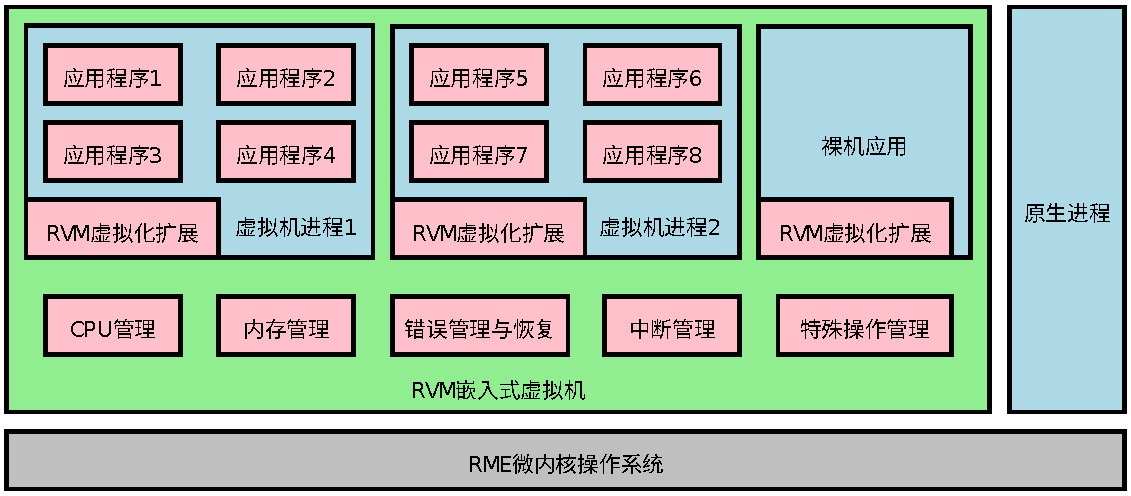
\includegraphics[width=0.90\textwidth]{Figure/image2.pdf}
\caption{RVM架构简图}\label{fig:2-1}
\end{figure}


RVM虚拟机运行在一个基于准虚拟化技术实现的虚拟机监视器上。它实现了虚拟化的所有基本功能：内存管理、CPU管理、中断向量虚拟化和虚拟机错误处理。关于这些实现的具体信息请参见下文所述。

\subsection{RME微内核}\label{subsec:2-1-1}

RME微内核作为RVM的底层支撑存在，负责向RVM提供基本的操作系统服务。其它一切运行在微控制器上的组件都是作为RME进程存在的。有关RME微内核，请参见相关内核文档。

\subsection{RVM虚拟机监视器}\label{subsec:2-1-2}

RVM虚拟机监视器负责具体的虚拟机管理工作，它作为II型虚拟机监视器运行在RME上。具体地，它将物理中断和事件源信号下发到各个虚拟机，并响应来自各个虚拟机的超级调用请求。在虚拟机遇到异常时，RVM还负责重启对应的虚拟机。虚拟机监视器包括五个守护线程：启动守护线程（Initialization
Daemon，INIT）、安全守护协程（Safety Daemon，SFTD）、时间守护协程（Timer
Daemon，TIMD）、向量守护协程（Vector
Daemon，VCTD）和超级调用守护线程（Hypercall
Daemon，HYPD），其中后三个协程，它们共同运行于虚拟化守护线程（Virtual
Machine Monitor Daemon，VMMD）之上。下文将对这五个守护线程加以一一介绍。

\subsubsection{启动守护线程INIT}\label{subsubsec:2-1-2-1}

INIT是RME在启动时创建的，由它负责初始化系统中的原生线程与虚拟机，并启动剩下的四个守护线程。在这一工作完成后，INIT即进入休眠，并仅在系统中无可运行的线程时被调度。它一旦被调度，就反复执行处理器休眠命令，令处理器进入低功耗状态以等待中断来临。

\subsubsection{安全守护协程SFTD}\label{subsubsec:2-1-2-2}

SFTD运行在系统的最高优先级\footnote{Kern\_Prio-1}，负责监控原生进程和虚拟机的运行。它平时阻塞在错误处理端点RVM\_Sftd\_Sig\_Cap上，一旦原生进程和虚拟机发生任何异常，SFTD便解除阻塞开始运行。若发生异常的是原生进程，SFTD将重启整个系统；若发生异常的是虚拟机，则SFTD仅重启该虚拟机。

\subsubsection{向量守护协程VCTD}\label{subsubsec:2-1-2-3}

VCTD运行在较原生进程低，但较虚拟机高的优先级上，负责将系统中的物理中断和事件激活转送给各个虚拟机的中断源。它平时阻塞在中断向量端点RVM\_BOOT\_INIT\_VCT上，一旦该端点收到任何信号，VCTD便解除阻塞开始运行。VCTD将从分别位于RVM\_PHYS\_VCT\_BASE和RVM\_VIRT\_EVT\_BASE的两个RVM\_Flag数据结构中提取中断向量和事件源激活信息，并将其转送给虚拟机。

每个RVM\_Flag数据结构都由两个相同的struct
\_\_RME\_RVM\_Flag合并而成。这是因为，VCTD访问struct
\_\_RME\_RVM\_Flag时需要独占它，而此时内核若需要传递激活信息给RVM，只能选择填充另一个结构体副本。每个结构体内部都有如下三个域：

\begin{xltabular}{\textwidth}{@{}>{\hsize=0.4500\hsize\raggedright\arraybackslash}X>{\hsize=1.5500\hsize\raggedright\arraybackslash}X@{}}
\caption{struct \_\allowbreak{}\_\allowbreak{}RME\_\allowbreak{}RVM\_\allowbreak{}Flag中各个域的意义}\label{tab:2-1}\\
\toprule
域名称 & 作用\tabularnewline
\endfirsthead
\toprule
域名称 & 作用\tabularnewline
\midrule
\endhead
\bottomrule
\endlastfoot
ptr\_\allowbreak{}t Lock &
决定此结构体是否正被VCTD使用。如果VCTD正在使用该结构体，内核无法对此结构体进行操作，否则可能引起竞争冒险。则内核会选择去填充另一个结构体。\tabularnewline
ptr\_\allowbreak{}t Fast &
指示快速信号源的激活。如果为1，则快速中断源激活。当前，这一个域仅在位于RVM\_\allowbreak{}PHYS\_\allowbreak{}VCT\_\allowbreak{}BASE的结构体中使用，用来传达时钟中断信号。\tabularnewline
ptr\_\allowbreak{}t Group &
指示被激活的慢速信号源的组别，是一个位图。若某位被置位，则意味着Flag域中该组别有被激活的信号：如果第2位被置位，则意味着Flag{[}2{]}的某一位不为0。设置该域的目的是快速查找被激活的信号所在的组别。\tabularnewline
ptr\_\allowbreak{}t Flag{[}{]} &
一个位图，指示具体的被激活的信号源。其长度由信号的数量决定：如果某处理器的字长为32位，而有96个中断源，则此域的长度为96/32=3个机器字长。\tabularnewline
\end{xltabular}

比如，在32位处理器上，若34号物理中断源被激活，内核会首先查找位于RVM\_PHYS\_VCT\_BASE的两个struct
\_\_RME\_RVM\_Flag结构体，并选择一个Lock域为0的副本。然后，内核会将Flag{[}1{]}的第{[}2{]}个位置位，并将Group的第{[}1{]}个位置位。最后，内核会向RVM\_BOOT\_INIT\_VCT发送信号，激活VCTD。VCTD被激活后，会交替查找两个struct
\_\_RME\_RVM\_Flag中存在的置位的位。它在查找时，首先将第一个struct
\_\_RME\_RVM\_Flag的Lock置1，然后查询Group中哪些位被置位，并根据该信息查询对应的Flag{[}{]}，得到具体的中断源编号。若激活的是34号中断源，则应当查询到Group的位{[}1{]}置位，并转去查询Flag{[}1{]}；在Flag{[}1{]}中则发现其位{[}2{]}置位。由此，VCTD可以推算出被激活的中断源是第34号，并将登记了34号物理中断源的那些虚拟机激活。有关虚拟机的激活，请参见\protect\hyperref[subsec:2-2-4]{2.2.4}
。

事件源的激活过程与物理中断源的激活过程是类似的。关于事件源，请参见\protect\hyperref[subsec:2-2-7]{2.2.7}
。

\subsubsection{时间守护协程TIMD}\label{subsubsec:2-1-2-4}

时间守护线程TIMD运行在与VCTD相同的优先级上，负责将RVM时钟嘀嗒传递给各个虚拟机。它平时阻塞在时钟中断端点RVM\_BOOT\_INIT\_VCT上，一旦该端点收到定时器中断就将该中断传递给所有虚拟机。TIMD每在时钟中断端点RVM\_BOOT\_INIT\_VCT上收到一次信号，就称作一个RVM时钟嘀嗒。每个虚拟机可以指定一个分频系数Period\footnote{请参见\protect4.2}，在收到Period个RVM时钟嘀嗒后才会向虚拟机发送一个虚拟时钟中断。

时间守护线程还允许为每个虚拟机指定一个看门狗超时时间Watchdog\footnote{请参见\protect4.2}。虚拟机可以使用超级调用RVM\_Hyp\_Wdg\_Clr来投喂看门狗；如果该虚拟机在Watchdog个时钟嘀嗒后仍未喂狗，则判断该虚拟机陷入死循环，此时TIMD将重启它。

\subsubsection{超级调用守护协程HYPD}\label{subsubsec:2-1-2-5}

超级调用守护线程HYPD运行在与VCTD相同的优先级上，负责接受并处理各个虚拟机发来的超级调用。它平时阻塞在超级调用处理端点RVM\_BOOT\_INIT\_VCT上，一旦该端点收到信号就处理当前虚拟机发起的超级调用。有关超级调用的具体处理方法，请参见\protect\hyperref[subsec:2-2-6]{2.2.6}
。

\needspace{14\baselineskip}
\subsection{保护域}\label{subsec:2-1-3}

\needspace{10\baselineskip}
RVM提供两种保护域，分别是原生进程和虚拟机。两者的简要对比如下：

\begin{xltabular}{\textwidth}{@{}>{\hsize=1.0000\hsize\raggedright\arraybackslash}X>{\hsize=1.0000\hsize\raggedright\arraybackslash}X>{\hsize=1.0000\hsize\raggedright\arraybackslash}X>{\hsize=1.0000\hsize\raggedright\arraybackslash}X>{\hsize=1.0000\hsize\raggedright\arraybackslash}X>{\hsize=1.0000\hsize\raggedright\arraybackslash}X>{\hsize=1.0000\hsize\raggedright\arraybackslash}X>{\hsize=1.0000\hsize\raggedright\arraybackslash}X>{\hsize=1.0000\hsize\raggedright\arraybackslash}X@{}}
\caption{原生进程与虚拟机的对比}\label{tab:2-2}\\
\toprule
保护域 & 秘密性 & 完整性 & 可用性 & 可审计性 & 实时性 & 紧凑性 & 可靠性
& 易用性\tabularnewline
\endfirsthead
\toprule
保护域 & 秘密性 & 完整性 & 可用性 & 可审计性 & 实时性 & 紧凑性 & 可靠性
& 易用性\tabularnewline
\midrule
\endhead
\bottomrule
\endlastfoot
原生进程 & 强 & 弱 & 弱 & 弱 & 强 & 强 & 弱 & 弱\tabularnewline
虚拟机 & 强 & 强 & 强 & 强 & 弱 & 弱 & 强 & 强\tabularnewline
\end{xltabular}

\subsubsection{原生进程}\label{subsubsec:2-1-3-1}

RME原生进程直接运行在RME微内核上，它们不受RVM虚拟机监视器的制约，且资源消耗要比虚拟机低。它们主要用来接受从中断向量来的信号，并在进行初步处理后将这些信号转发给虚拟机。原生进程内的线程的时间片都是无限的，且在整个系统中拥有最高的优先级。即使RVM和它负责管理的所有虚拟机都已崩溃，原生进程内的线程仍能正常运行，从而维护被控设备的安全。

即便原生进程不是虚拟机，工程生成器仍对它们提供了完善的支持，RVM的用户态库也提供一系列对系统调用的封装以方便在C程序中使用系统调用。工程生成器甚至可以生成不含虚拟机的工程，此时只能使用原生进程和系统调用来完成应用程序的功能。

RVM没有为原生进程提供容错功能；如果任何一个原生进程发生异常，则RVM的SFTD将认为系统中出现了严重的问题，并重启整个系统。因此，原生进程仅具备安全三要素中的秘密性，一旦被入侵，则系统的完整性和可用性将荡然无存。

\subsubsection{虚拟机}\label{subsubsec:2-1-3-2}

每个RVM虚拟机都是一个单独的进程，其内部可以模拟RTOS运行时依赖的硬件抽象层。它具备一个中断向量线程Vct和一个用户程序线程Usr来分别模拟处理器中断和正常的程序执行流：为方便RTOS的软中断线程切换，Usr线程可以直接触发Vct线程的运行，且Vct线程可以直接修改Usr线程的寄存器组。

在基于RVM的系统中，推荐将任何稍复杂的功能，尤其是那些语言虚拟机、图形界面等放置在虚拟机中实现。这不仅是因为虚拟机中的RTOS提供了一系列库、可能的POSIX支持和已认证的软件，更是因为虚拟机在发生故障后仅会自动重启自身而非整个系统。这对于功能安全中的故障隔离是至关重要的。

虚拟机可以通过超级调用来访问一系列与虚拟化相关的特殊功能，包括中断管理、事件源管理与通信等。这些超级调用将被RVM的HYPD拦截并响应。

\subsection{工程生成器}\label{subsec:2-1-4}

RVM提供的工程生成器能够根据工程描述文件生成可编译的工程。它能够自动计算并分配各个内核对象的地址，并生成对应的配置文件，无需用户做任何手动调整。

\section{虚拟化原理}\label{sec:2-2}

在RVM启动后，第一个执行的是启动守护线程INIT。它会加载各个虚拟机。并负责启动安全守护线程、向量守护线程、超调用守护线程和时间守护线程。其中，安全守护线程会在虚拟机发生错误时重启它\footnote{RVM不原生支持用户自定义错误处理}，向量守护线程会把来自设备的物理中断或事件源的激活重定向给对应虚拟机的虚拟中断向量，超调用守护线程负责处理超级调用和虚拟机调度；时间守护线程则负责向各个虚拟机发送时钟中断。

每一个虚拟机内部则运行两个线程，一个负责处理虚拟机内部的中断，另一个则负责运行用户代码。具体的虚拟化原理会在以下各小节分别介绍。

\subsection{优先级配置}\label{subsec:2-2-1}

在RVM中，安全守护线程SFTD永远运行在系统的最高优先级。紧随其后的是原生进程中的线程，它们负责快速处理系统中的部分来不及发送给虚拟机处理的中断。再接下来是VCTD、TIMD和HYPD三个守护线程，它们运行在比原生进程低但比虚拟机高的优先级上。然后则是在运行的虚拟机的中断处理线程Vct和用户线程Usr，其中Vct的优先级又要高于Usr。再之后是系统本身的INIT进程，该进程负责无限循环调用空闲钩子，在没有虚拟机就绪时让系统进入休眠。最后则是未在运行的虚拟机的中断处理线程和用户程序线程。整个虚拟化体系的各线程的中断优先级如下所示：


\begin{figure}[htbp]
\centering
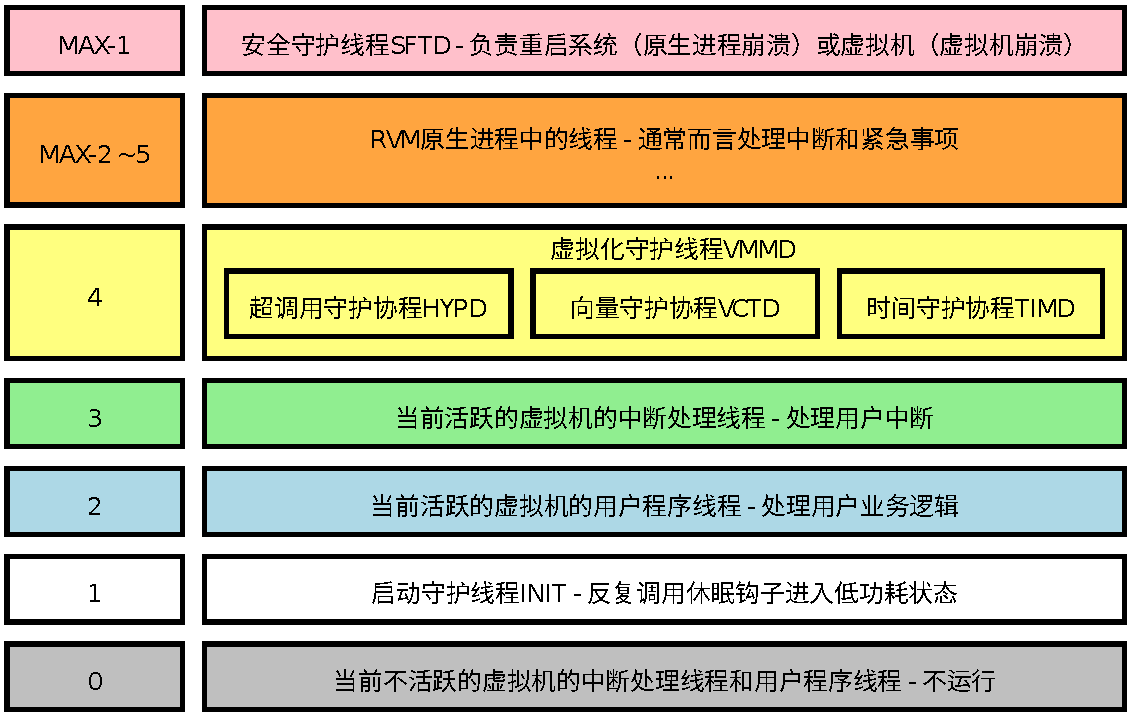
\includegraphics[width=0.90\textwidth]{Figure/image3.pdf}
\caption{虚拟化体系的中断优先级}\label{fig:2-2}
\end{figure}


各个虚拟机采用固定优先级时间片轮转法调度。它们之间的优先级则是由调度器守护线程决定的。为了系统安全，虚拟机的时间片和优先级是在系统编译时静态决定好的，RVM并不提供可以修改这两点的超级调用。这从根本上保证了虚拟机之间的时间隔离，使得没有虚拟机可以破坏整个系统的实时性。

\subsection{内存管理}\label{subsec:2-2-2}

在虚拟机中，最重要的事项之一就是内存管理。考虑到微控制器应用的一般特点，每个虚拟机的私有内存和共享内存，都是在编译时静态指定的。在系统开始运行之后，不再允许修改内存映射。对于每一种处理器，页表信息的格式都是不同的。请参看相应处理器的使用手册确定该处理器的页表形式。

手动构造和填充页表是非常繁琐的；为了避免不必要的麻烦，工程生成器提供了页表自动构造和填充的相关功能。

\subsection{CPU的虚拟化}\label{subsec:2-2-3}

在不同的准虚拟化平台中，CPU的虚拟化主要有两种主流设计策略，分别如下：

\begin{enumerate}
\def\labelenumi{{[}\arabic{enumi}{]}}
\item
  将每个虚拟机作为一个线程运行。这是专用准虚拟化平台最常见的解决方案，Xen即采取该策略。在每个客户机中，线程平时执行应用程序的代码；一旦设备中断或异常发生\footnote{在x86上，Xen利用了硬件特有的Ring1来加速系统调用和异常的处理，并不经过Xen，但设备中断依然需要经过Xen进行分发}，虚拟机监视器即强制修改线程的执行地址，迫使其执行一段中断处理代码，待处理结束后该线程自行返回应用程序中执行。在虚拟机监视器看来，此种方法最为方便，一方面每个客户机只有一个执行上下文，另一方面激活中断只要修改该上下文的指令指针。然而，在客户机看来，中断结束（End-Of-Interrupt，EOI）是否需要特意通知虚拟机监视器的问题会变得很难处理。这里主要有两种情况：相对简单的（1）虚拟机监视器一旦迫使某客户机执行虚拟中断向量，在客户机使用专用的超级调用通知虚拟机监视器当前中断已结束之前，虚拟机监视器不得再修改指令指针以迫使虚拟机执行中断向量，和较为复杂的（2）虚拟机监视器会无视客户机是否正在执行虚拟中断向量而总是修改指令指针迫使虚拟机执行中断向量。在情况（1）中，客户机端需要调用超级调用来通知虚拟机，这无疑增加了一次超级调用。对于直接运行在特权态的原生型虚拟机监视器Xen而言，一次超级调用就是一次上下文切换，开销还是可以忍受的；对于运行在用户态的宿主型虚拟机监视器RVM而言，一次超级调用意味着两次上下文切换，引入的延迟就不可忽视了。如果采取情况（2）中的解决方案，则更加糟糕：这意味着中断向量入口是必须可重入的，因此需要一段非常特殊的汇编代码。这段代码必须负责在重入的执行实例执行到真正的中断向量之前识别重入且在此后主动退出，在退出的过程中还要涉及对栈框的修补以使执行流带着正确的栈指针返回正在执行的中断向量。一方面这段代码非常难以正确编写\footnote{对五花八门的非标准嵌入式架构就更是如此}，另一方面它的开头总是大片的压栈。如果发生一系列紧密连续的中断，开头的压栈代码就会在来得及进行栈框修补之前重入多次，在嵌入式环境下会导致潜在的栈溢出。因此，即便（2）在Xen中非常高效，我们也不采用这种方式。
\item
  将每个客户机中的每个线程都作为一个独立的虚拟机线程运行。这是基于微内核的虚拟化的常见方案，L4Linux即采用该策略\protect\hyperref[cite:2-2]{{[}2{]}}。在微控制器上，这种策略的问题是（1）需要将原客户机操作系统的线程接口想办法对接到微内核的系统调用，这需要充分理解原操作系统的设计，甚至可能涉及到线程控制块等架构不相关部分的修改，（2）将每一个客户机线程都对应到微内核线程会导致创建出大量的微内核线程对象，这在Linux等线程结构本就庞大的重量级操作系统中是没有问题的，但在线程普遍极为轻量的RTOS中就等于成倍放大了存储器消耗，（3）微内核的线程切换需要经过一系列操作权能检查、时间预算检查和保护域切换检查，而甚至不具备保护域的RTOS线程根本用不着这些检查，每次都调用微内核系统调用来进行线程切换相当于成倍放大了执行时间消耗，在那些把时间资源作为独立可分配资源的微内核\footnote{如Composite和某些L4变体等}上就更是如此。

  为了解决上面的困境，RVM采用双线程的方法进行客户机的CPU虚拟化。每个客户机都具有Vct和Usr两个线程，Vct线程负责中断处理，Usr线程则负责处理用户程序。Vct平时不运行，只有当接收到了来自RVM的中断触发信号时才运行。当中断处理完成后，Vct又阻塞，Usr开始运行。Vct到Usr的切换利用了微内核的高效异步信号机制，不涉及RVM，因此比超级调用快得多。

  在Usr被切换走时，其寄存器组会被保存在由Reg\_Base\footnote{请参见\protect4.2}指定的地址。因此，要在Vct中修改Usr的寄存器组，只要修改那个地址上的寄存器数据即可。利用这个方法，可以在无需理解原RTOS设计的基础上对其硬件抽象层、尤其是其线程切换汇编进行逐行替换，从而轻松模拟RTOS中非常常见的线程上下文切换。
\end{enumerate}

\subsection{中断的虚拟化}\label{subsec:2-2-4}

对于虚拟机而言，中断虚拟化是必不可少的。RVM的每个客户机中都具有一个中断处理线程Vct，该线程的优先级比处理用户程序的Usr线程要高。该线程平时阻塞在各个虚拟机专属的虚拟中断向量端点上\footnote{该端点在每个虚拟机内部都位于权能号1的位置}，直到收到RVM发来的虚拟中断信号才被唤醒运行。

系统中的中断大概可以分成三类，第一类是时钟中断，它负责向操作系统提供时钟嘀嗒；第二类是线程切换中断，它负责进行RTOS的线程切换；第三类则是其他系统中断，它们负责响应其他外设的事务。这三类中断的特点也不同：时钟中断是周期性频繁发生的；线程切换中断本质上是自己发送给自己的软中断；其他系统中断则是不时发生的无规律中断。因此，RVM对于这三种中断采取了不同的虚拟化策略。

每个虚拟机都维护一个RVM\_State数据结构，其地址被State\_Base\footnote{请参见\protect4.2}指定。其内部的域如下：

\begin{xltabular}{\textwidth}{@{}>{\hsize=0.4500\hsize\raggedright\arraybackslash}X>{\hsize=1.5500\hsize\raggedright\arraybackslash}X@{}}
\caption{struct RVM\_\allowbreak{}State中各个域的意义}\label{tab:2-3}\\
\toprule
域名称 & 作用\tabularnewline
\endfirsthead
\toprule
域名称 & 作用\tabularnewline
\midrule
\endhead
\bottomrule
\endlastfoot
ptr\_\allowbreak{}t Vct\_\allowbreak{}Act &
指示当前虚拟机中运行的线程。如果置1，说明Vct线程正在运行，否则说明Usr线程正在运行。\tabularnewline
struct RVM\_\allowbreak{}Param Vct & Vct线程专用的超级调用参数区。\tabularnewline
struct RVM\_\allowbreak{}Param Usr & Usr线程专用的超级调用参数区。\tabularnewline
struct RVM\_\allowbreak{}Vctf Flag &
指示当前虚拟机中被激活的虚拟中断向量。\tabularnewline
\end{xltabular}

在该数据结构中，与中断虚拟化相关的数据结构为struct RVM\_Vctf Flag，它的各个域如下表所示。关于其它域，请参见\protect\hyperref[subsec:2-2-6]{2.2.6}
。

\begin{xltabular}{\textwidth}{@{}>{\hsize=0.4500\hsize\raggedright\arraybackslash}X>{\hsize=1.5500\hsize\raggedright\arraybackslash}X@{}}
\caption{struct RVM\_\allowbreak{}Vctf中各个域的意义}\label{tab:2-4}\\
\toprule
域名称 & 作用\tabularnewline
\endfirsthead
\toprule
域名称 & 作用\tabularnewline
\midrule
\endhead
\bottomrule
\endlastfoot
ptr\_\allowbreak{}t Tim & 指示时钟中断激活。\tabularnewline
ptr\_\allowbreak{}t Ctx & 指示线程切换中断激活。\tabularnewline
u8\_\allowbreak{}t Vct{[}{]} &
指示其它虚拟中断向量激活。每个字节对应一个虚拟中断向量。\tabularnewline
\end{xltabular}

在该数据结构中，时钟中断和线程切换中断的激活由两个单独的机器字指示，其它虚拟中断向量则每个对应于一个字节。当对应的中断被激活时，相应的域就被置1。这里不采取一个二进制位对应一个中断向量的方法，这样就不需要原子逻辑与指令\footnote{VCTD在置位某个向量时，Vct线程可能正在复位其中的某个向量。如果采取每个二进制位对应一个中断向量，则Vct线程必须使用原子逻辑与操作来复位标志位。部分架构，如ARMv6-M，是没有这种原子操作的，因此一个字节对应一个标志兼容性更好。}。由于每个虚拟机的虚拟中断向量数都有限，所以造成的存储空间浪费是可以容忍的。

比如，若VCTD判定某虚拟机的4号中断向量被激活，它会将Vct{[}4{]}置1，并向该虚拟机的Vct线程的专属端点发送信号。收到该信号的Vct线程被激活后，会先扫描整个结构体，并通过Vct{[}4{]}被置1判断4号虚拟中断向量被激活。之后，Vct线程会先将Vct{[}4{]}清零，再调用用户使用RVM\_Virt\_Vct\_Reg\footnote{请参见\protect4.5.5}注册的4号虚拟中断向量。这样一来，即便用户注册的中断向量执行时有新的4号中断到来，也不会产生中断丢失，因为Vct{[}4{]}将重新置位：Vct线程将在下一个循环后检测到4号中断悬起并再次进入它。

虚拟机的中断开关，以及虚拟机的虚拟中断向量与对应物理中断向量或事件源的对应关系是可以通过超级调用设置的。有关这些超级调用的信息请参见\protect\hyperref[sec:4-4]{4.4}
。一个标准的虚拟机中断初始化流程是：

\begin{enumerate}
\def\labelenumi{{[}\arabic{enumi}{]}}
\item
  调用RVM\_Virt\_Tim\_Reg注册时钟中断，
\item
  调用RVM\_Virt\_Ctx\_Reg注册线程切换中断，
\item
  调用RVM\_Virt\_Vct\_Reg注册其它虚拟中断，
\item
  调用RVM\_Hyp\_Vct\_Phys将所需的物理中断源映射到虚拟中断源，
\item
  调用RVM\_Hyp\_Vct\_Evt将所需的事件源映射到虚拟中断源，
\item
  调用RVM\_Hyp\_Vct\_Lck将事件源映射锁死以防止后续篡改，
\item
  在合适的地方调用RVM\_Hyp\_Int\_Ena开启虚拟机总中断。如果虚拟机还使用看门狗，需要调用RVM\_Hyp\_Wdg\_Clr来启动看门狗。看门狗一经启动则无法关闭。
\item
  虚拟机内的RTOS在其空闲线程中应当反复调用RVM\_Hyp\_Vct\_Wait以使虚拟机在空闲时进入休眠，并等待下一次中断来临。如果虚拟机还使用看门狗，需要在合适的地方调用RVM\_Hyp\_Wdg\_Clr来喂狗。
\end{enumerate}

\subsubsection{定时器中断的虚拟化}\label{subsubsec:2-2-4-1}

在RVM上运行的RTOS按照对定时器的运用方式可以分为两类，分别是有节拍（Periodic）内核和无节拍（Tickless）内核。前者要求系统中具备一个周期性发送中断的自动重装（Auto-reload）定时器，后者则要求每次上下文切换时按需编程一个倒计时结束后发送中断的一次性（One-shot）定时器。在裸机上，后者在低功耗特性方面更加优越，因为在处理器休眠或仅调度一个任务时不产生时钟中断。为此，在那些支持无节拍内核的RTOS上，我们常常启用这个特性。

然而，在虚拟化环境中则正好相反。无节拍内核对定时器的编程不再能直接完成，而要通过超级调用求助RVM。这会导致在每次上下文切换时多出一个超级调用，从而造成难以忍受的性能和实时性开销。此外，并非所有的RTOS都支持无节拍内核模式：哪怕有一个有节拍内核运行在RVM上，RVM还是要周期性地被唤醒以发送定时器中断给它，从而不可能降低功耗；这让其它内核的无节拍特性变得徒增开销。退一步讲，即便运行在RVM上的一切虚拟机都是无节拍的，它们对定时器的编程次数的总和也会非常多，而RVM必须将硬件定时器的超时时间设置成所有时刻中的最小值。这会导致定时器总是在一小段时间后就被触发，也不太可能起到低功耗效果。

基于上述原因，RVM使用有节拍设计。它需要的周期性时钟信号由RME的底层定时器产生，并且通过RVM\_BOOT\_INIT\_TIM端点发送到RVM的时钟处理守护线程。该守护线程会计算当前经过的时间周期数，并且根据各个虚拟机配置的分频系数Period\footnote{请参见\protect4.2}给各个虚拟机发送时钟中断。

具体地，Vct线程将调用用户使用RVM\_Virt\_Tim\_Reg\footnote{请参见\protect4.5.7}注册的线程切换钩子Tim。该钩子函数可以直接使用原裸机RTOS的定时器中断向量，且在需要时可使用RVM\_Virt\_Yield\footnote{请参见\protect4.5.7}来触发上下文切换\footnote{就好像在原RTOS中触发PendSV等上下文切换中断那样}。

\subsubsection{线程切换中断的虚拟化}\label{subsubsec:2-2-4-2}

线程切换中断本质上是一个软中断，它来源于虚拟机自身的内部。这个中断的响应效率将直接决定虚拟机的线程切换时间，因此保证它的效率非常重要。为此，RVM被特别设计为可以由用户线程Usr在不经过虚拟机监视器介入的情况下使用RVM\_Virt\_Yield\footnote{请参见\protect4.5.7}直接触发Vct线程主导的上下文切换，且在Vct线程中可直接修改提前映射到Reg\_Base\footnote{请参见\protect4.2}的Usr寄存器组，无需再使用任何系统调用。这个实现最大限度地贴近了常见RTOS的线程切换语义，大大降低了虚拟机内部的线程切换开销。

具体地，Vct线程将调用用户使用RVM\_Virt\_Ctx\_Reg\footnote{请参见\protect4.5.7}注册的线程切换钩子Ctx。在该钩子中将实现对Usr的各个寄存器的保存和恢复，从而完成RTOS线程的切换。常见的线程切换手段包括两个步骤，（1）将一切寄存器压到老线程栈上，（2）再从新线程栈上恢复一切寄存器；这个过程在裸机RTOS中通常是由汇编语言完成的。在RVM中，实现该流程的Ctx钩子则可由C语言写成\footnote{具体例子可以参见RMP的RVM移植}。

与裸机RTOS不同，寄存器的保存和恢复必须包括Usr线程使用的超级调用参数缓冲区，它位于struct
RVM\_State结构体的struct RVM\_Param
Usr域。这是因为，Usr线程对应的多个RTOS线程可能会并发访问它\footnote{比如它们同时进行超级调用}。关于该域的详细信息，请参见\protect\hyperref[subsec:2-2-6]{2.2.6}
。

\subsubsection{其他中断的虚拟化}\label{subsubsec:2-2-4-3}

由于不同的虚拟机需要接收不同的外设中断，因此其他外设中断要按需送往各个虚拟机。因此，系统提供了调用接口来让各个虚拟机设置自己的每个虚拟中断向量对应的物理中断源。每个虚拟机能且只能设置自己的虚拟中断向量对应的物理中断源。一旦该物理中断被触发，登记于这个物理中断上的所有的虚拟机的相应虚拟中断向量均会收到此中断。虚拟中断源的编号越小，其优先级就越高，但虚拟中断之间不会发生抢占和嵌套。

各虚拟中断对应的中断处理向量可以注册为不可掩蔽的``透明中断''或可掩蔽的``可感知中断''\footnote{这模拟了ARMv7-M等的PRIMASK功能，允许客户机在锁调度器时响应与RTOS无关的中断，提高了实时性}。前者在中断被掩蔽时仍会被响应，后者在中断被掩蔽时则不会被响应。定时器中断和线程切换中断则总是可掩蔽的。有关这些超级调用的信息，请参见\protect\hyperref[sec:4-4]{4.4}
。

\subsection{设备的虚拟化}\label{subsec:2-2-5}

在不同的虚拟化平台中，设备及其驱动的虚拟化主要有四种主流设计策略，分别如下：

\begin{enumerate}
\def\labelenumi{{[}\arabic{enumi}{]}}
\item
  将设备驱动放进一个单独的、具备特权虚拟机Dom0中，其余虚拟机通过向该虚拟机发送请求来访问设备。这是Xen等原生型虚拟机监视器常采取的策略\protect\hyperref[cite:2-1]{{[}1{]}}。采取这种策略的动力很好理解：（1）将设备直接交给虚拟机是无法安全共享的，要将它们与虚拟机隔离就需要将其放进单独的保护域，而虚拟机监视器提供了虚拟机作为隔离手段，（2）客户机操作系统中已有现成的驱动，单独为虚拟机监视器再准备一套驱动无异于重造轮子。然而，这种策略使任何设备I/O都包含昂贵的虚拟机间上下文切换，性能开销极大。此外，一旦虚拟机监视器对Dom0的中断调度或分发不当，其延迟将会扩散到整个系统中，造成毁灭性的实时性问题\protect\hyperref[cite:2-3]{{[}3{]}}。因此，RVM不能采取这种策略。
\item
  将设备驱动放在虚拟机监视器所在的内核态中。这是VMware ESXi等原生虚拟机监视器采取的另一种策略。这种方案可以完全规避掉Dom0的性能问题，但它将虚拟机监视器------也即整个系统的可信计算基------置于恶意驱动的威胁之下。显然，只有在虚拟机监视器厂商对驱动非常自信的情况下才能这样做，而且第三方设备厂商还必须配合这种认证。在微控制器中这些条件都不存在，因此RVM不能采取这种策略。
\item
  将虚拟机监视器和操作系统内核做成一个，这样客户机自然就能享受操作系统自带的设备驱动。这是KVM等虚拟机监视器通常采取的策略。它和上一种策略实际上或多或少是同样的，只不过驱动程序的开发者普遍认为开发工作是给Linux做的，因而积极性相对较高。
\item
  将各个驱动程序直接放置在各客户机中。这是很多工业场景和功能安全场景下的解决方案，因为工业场景下的每个虚拟机往往是各司其职\footnote{可以说是沿功能的分界面进行``纵切''，而非像大多数系统那样沿抽象层次的分界面进行``横切''}，各客户机间的功能重叠面很小，硬件的共享面也很小。利用工业嵌入式场景的这个特性，这个方案在设备划分得当时往往非常高效，因为虚拟机监视器将不再介入除中断分发之外的任何设备操作。然而，这种方案要求（1）任何设备的错误甚至是恶意操作都不得对系统安全和实时性造成威胁，包括那些往往被忽视的、由侧信道引起的问题\footnote{最典型的是DMA控制器，允许不可信虚拟机任意操作它可以轻易绕过所有安全机制}，（2）任何设备都只能被一个虚拟机独占，无法在虚拟机间进行任何设备共享，而且（3）中断仍然要传递到虚拟机中才可以处理，实时性不够。因此，这种方案不是总能使用。

  考虑到微控制器的实际情况，RVM鼓励在任何可能的时候使用方案4。如果实时性不够，或者需要共享设备，可以考虑将驱动程序的简单、可信赖的上半部\footnote{通常只包括寄存器的简单读写以及消息队列的发送}放置在中断响应极快的原生进程中，而将其下半部和协议栈放置在客户机中。原生进程可以和客户机都共享一部分内存以用于传递数据，且在共享时要保证客户机不破坏原生进程中线程执行所必要的数据。
\end{enumerate}

\subsection{超级调用的设计}\label{subsec:2-2-6}

虚拟机可以通过超级调用向虚拟机监视器请求服务。有关这些超级调用的信息，请参见\protect\hyperref[sec:4-4]{4.4}
。要发起超级调用，虚拟机会先将超级调用所需的各个参数写到与RVM约定好的参数缓冲区，然后向HYPD的信号端点RVM\_Hypd\_Sig\_Cap发送信号\footnote{该端点在每个虚拟机内部都位于权能号0的位置}。该参数缓冲区位于RVM\_State数据结构中，且存在两份：struct
RVM\_Param Vct为Vct线程专用，而struct RVM\_Param
Usr为Usr线程专用，这样就可以防止Vct线程和Usr线程在参数缓冲区上产生竞争冒险。

HYPD在收到超级调用后，会通过RVM\_State数据结构中的Vct\_Act判断当前正在运行的线程。如果Vct\_Act为1，说明当前运行的是Vct线程，超级调用参数应当从Vct线程的参数缓冲区中提取；否则说明当前运行的是Usr线程，超级调用参数应当从Usr线程的参数缓冲区中提取。在执行完超级调用之后，HYPD会将返回值写回对应的参数缓冲区；虚拟机在重新获得运行权后将提取该值作为超级调用的返回值。

由于一个Usr线程对应的多个RTOS线程同时也可能并发访问Usr线程的参数缓冲区，因此在RTOS的线程切换中，Usr线程使用的参数缓冲区将和寄存器组一起压栈弹栈，这确保了不会发生竞争冒险。

\subsection{跨保护域通信}\label{subsec:2-2-7}

为安全起见，原生进程与原生进程之间、原生进程与虚拟机之间，以及虚拟机与虚拟机之间是默认无法互相发送信号的。要使它们可以互相通信，需要做一些配置以在各个保护域中置入合适的信号原语。

\subsubsection{从原生进程发送信号到原生进程}\label{subsubsec:2-2-7-1}

原生进程之间可以通过RME的异步信号机制来进行通信。一个进程中的线程在信号端点上阻塞后，另一个进程中的线程只要向该端点发送信号就可以将阻塞解除。这要求一个进程具备端点的接收权能，另一个进程具备端点的发送权能。相关信息请参见\protect\hyperref[subsec:3-5-6]{3.5.6}
。

工程生成器可以根据用户对原生进程的描述正确地生成这种权能布局。只需要在接收的进程中声明接收端点，然后在发送的进程中向该端点发送就可以了。

\subsubsection{从虚拟机发送信号到原生进程}\label{subsubsec:2-2-7-2}

若要从虚拟机发送给原生进程，则可直接在原生进程中声明接收信号端点，并在虚拟机中声明发送信号端点，由虚拟机直接向原生进程发起信号发送即可。相关信息请参见\protect\hyperref[subsec:3-5-6]{3.5.6}
。

工程生成器允许在虚拟机中引用任何原生进程中声明的接收端点，并能够在系统启动时将对应的端点发送权限正确赋予虚拟机；虚拟机只需要向该端点发送就可以了。

\subsubsection{原生进程或虚拟机发送信号到虚拟机}\label{subsubsec:2-2-7-3}

由于虚拟机的Vct和Usr线程是不允许阻塞在信号端点上的，虚拟机内也无法定义信号端点发送权限之外的任何其它内核对象，从其它保护域\footnote{无论该保护域是原生进程还是虚拟机}到虚拟机的通信只能采取激活虚拟中断的方法。为此，RVM引入了``事件源''的概念\footnote{和常规的物理中断源一样，事件源也是一种全局刺激来源}：每个虚拟机都可以将自己的虚拟中断向量通过RVM\_Hyp\_Vct\_Evt自由注册到事件源，该事件源一旦激活，注册了该中断源的虚拟机就都会收到该虚拟中断。

原生进程的优先级高于虚拟机，因此限制它们对事件源的发送没有意义\footnote{它们只需要一直抢占处理器就可以阻止虚拟机监视器以及虚拟机的运行，因此限制它们没有意义}。虚拟机与虚拟机之间则并非如此：在虚拟机启动后，首先要通过RVM\_Hyp\_Evt\_Add函数事先申请向事件源进行发送的权限，并在申请完成后使用RVM\_Hyp\_Vct\_Lck将所有的事件源发送权限\footnote{以及事件源/中断源到虚拟中断之间的映射关系}锁死，在锁死后则不再允许对权限进行任何修改。此设计是基于这样一个假设：此后，通过RVM\_Hyp\_Evt\_Snd即可向事件源进行发送。相关信息请参见\protect\hyperref[sec:4-4]{4.4}
。

若要从虚拟机发送给原生进程，则可直接在原生进程中声明接收信号端点，并在虚拟机中声明发送信号端点，由虚拟机直接向原生进程发起信号发送即可。有关这些函数，请参见\protect\hyperref[subsec:3-5-6]{3.5.6}
。

事件源的总数量和事件源/物理中断源到虚拟中断的映射总数在工程生成器中可以配置，它是在工程编译前就静态决定好的；具体的映射关系则是在运行时动态建立的。

\needspace{12\baselineskip}
\section{本章参考文献}\label{sec:2-3}

\begin{enumerate}
\def\labelenumi{{[}\arabic{enumi}{]}}
\item
  \protect\phantomsection\label{cite:2-1}
  D. Chisnall, \textit{The Definitive Guide to the Xen Hypervisor}.
  Prentice Hall Open Source Software Development Series. Upper Saddle
  River, NJ, USA: Prentice Hall, 2008.
\item
  \protect\phantomsection\label{cite:2-2}
  A. Lackorzynski, ``L4Linux porting optimizations,'' Master's thesis.
\item
  \protect\phantomsection\label{cite:2-3}
  S. Yoo, K.-H. Kwak, J.-H. Jo, and C. Yoo, ``Toward under-millisecond
  I/O latency in Xen-ARM,'' in \textit{Proceedings of the Second
  Asia-Pacific Workshop on Systems}, Shanghai, China: ACM, 2011.
\end{enumerate}

